% =============================================================================
% CAPÍTULO 8 — travessia (AGENTS.md §6): F1, o vigia vê dependência?
%
% O fracasso que o abre, com número na mão: uma mudança que existe só no par de duas séries não
% move a margem de nenhuma delas (0,0528 para 0,0523 e 0,0520 para 0,0513) e multiplica a
% contagem conjunta por quase quatro (0,41 para 1,56). O instrumento que vê paga em latência:
% 354 dias no orçamento mais falador, contra os 7 a 149 dias do vigia de margem.
%
% Medição: lab/experimentos/E09_dependencia_vigiada.ipynb. Figura: figuras/E09_dependencia_vigiada_1.pdf.
% =============================================================================

\chapter{O vigia não vê o que não está na série}
\label{cap:dependencia_vigiada}

\section{A primeira travessia}

Quatro voltas ensinaram a medir uma série: o corte, o orçamento, a célula do calendário, a
estatística que estima e a que anuncia, e o conjunto de explicações que sobrevivem ao dado. Tudo
isso tem uma coisa em comum, e é o que a travessia vem testar: \textbf{cada instrumento lê uma margem},
e algumas mudanças não estão em margem nenhuma.

A primeira pergunta é a mais direta das cinco que a travessia carrega. Um vigia construído para
olhar uma série consegue ver uma mudança que existe apenas \textbf{entre} duas? O capítulo da
dependência já mostrou que as coisas ruins vêm juntas mais do que a independência prevê; o que
este capítulo mede é outra coisa: se o vigia que este livro construiu detecta o dia em que elas
passam a vir juntas.

O fracasso tem forma exata, e vale escrevê-la antes de medi-la: ao proteger cada perna no seu
próprio corte, a proteção de cada uma continua a mesma, e a proteção conjunta muda. Nada muda em
nenhuma das duas séries. Tudo muda no que se pode perder junto.

\section{A construção}

A pergunta é sobre estrutura e não sobre o mundo (o contrato do projeto, seção oito), e por isso a mudança é posta de
propósito: duas pernas com a mesma lei, \numVizinhancaDias{} dias, e no dia
\numVizinhancaQuando{} só o pareamento muda --- a correlação entre elas vai de
\numVizinhancaRhoAntes{} a \numVizinhancaRhoDepois.

Cada margem fica idêntica do começo ao fim, por construção: mesma lei, mesmo tamanho, e o mesmo
sorteio. É o que faz desta uma pergunta de travessia --- o objeto de uma família medido com o
instrumento de outra ---, e é também o que torna o resultado inevitável de um lado e aberto do
outro.

\section{A margem é cega, e não por calibração}

O primeiro instrumento é o que o orçamento do alarme e o calendário construíram: o corte no décimo terceiro pior dos
últimos \numCorteJanela{} pregões, e as violações contadas dia a dia.

Aplicado às duas pernas, antes e depois do dia da mudança, ele dá isto: \numVizinhancaTaxaAAntes{}
na primeira perna antes e \numVizinhancaTaxaADepois{} depois; \numVizinhancaTaxaBAntes{} na segunda
antes e \numVizinhancaTaxaBDepois{} depois. A variação é de quatro décimos de milésimo na primeira perna e de sete na segunda.

A leitura desse número não é que o vigia é insensível, nem que está mal calibrado. É que ele não
tem o que ver: as duas séries que ele observa são \textbf{as mesmas} antes e depois, e a mudança vive
no par. Nenhum ajuste de limiar, janela ou orçamento cria informação onde ela não está. O
refutador desta pergunta --- a mudança de dependência sendo detectada pelo vigia de margem, sem
instrumento extra --- cai por aritmética, e não por medição.

\section{O instrumento que vê, e o que ele cobra}

O instrumento que vê já existe desde o capítulo da dependência: contar os dias em que as \textbf{duas}
pernas rompem o próprio corte, em blocos móveis, e comparar com o que a independência previria. A
mesma contagem, aqui, antes e depois do dia da mudança: \numVizinhancaConjuntoAntes{} por bloco
antes, \numVizinhancaConjuntoDepois{} depois.

Ele vê. E, como todo instrumento deste livro, cobra --- e a cobrança tem a mesma forma da do
orçamento do alarme, medida agora para a dependência.

\begin{table}[htbp]
  \centering
  \footnotesize
  \begin{tabular}{lrrr}
    \hline
    limiar & orçamento & latência mediana & mundos em que não viu \\
    (dias por bloco) & (anos por alarme) & (dias) & (de \numVizinhancaSementes) \\
    \hline
    dois & \numVizinhancaLimiarDoisAnos & \numVizinhancaLimiarDoisLatencia & nenhum \\
    três & \numVizinhancaLimiarTresAnos & \numVizinhancaLimiarTresLatencia & nenhum \\
    quatro & não soa em mundo parado & \numVizinhancaLimiarQuatroLatencia & \numVizinhancaLimiarQuatroNaoViu \\
    cinco & não soa em mundo parado & --- & \numVizinhancaLimiarCincoNaoViu \\
    seis & não soa em mundo parado & --- & \numVizinhancaLimiarSeisNaoViu \\
    \hline
  \end{tabular}
  \caption{O orçamento e a latência do instrumento conjunto, com a mudança acontecendo no meio da
    série. O orçamento é medido no mundo em que o par não muda, e a latência no mundo em que ele
    muda.}
  \label{tab:vizinhanca}
\end{table}

Lida de baixo para cima, a tabela diz o essencial. A partir do limiar quatro o mundo em que nada
muda \textbf{não produz o evento} dentro dos seis mil dias observados, e o orçamento deixa de ser
estimável nesta amostra --- o que não quer dizer que ele seja infinito, e o capítulo declara a
diferença. E no limiar mais falador que se conseguiu calibrar, um alarme a cada
\numVizinhancaLimiarDoisAnos{} anos, a latência é de \numVizinhancaLimiarDoisLatencia{} dias.

\section{A comparação que dá sentido ao número}

Um ano pode parecer pouco ou muito, e sozinho ele não diz. O contraste é o vigia de margem do
orçamento do alarme, com um alarme por ano: ali, a mudança que vem pela cauda é vista em
\numFormaDegrauDias{} dias, a que se aproxima em rampa em \numFormaRampaDias, e a deriva na média
em \numFormaDerivaDias.

O instrumento da dependência, no seu orçamento mais falador, leva
\numVizinhancaLimiarDoisLatencia{} dias. Ele é mais caro que o instrumento de margem por um fator
que vai de duas vezes e meia a cinquenta vezes, conforme a forma da mudança com que se compare --- e o
orçamento dele já é mais silencioso que o do vigia de margem, de modo que a comparação é generosa
com ele.

Vale dizer o que isso significa sem anestesia: \textbf{a dependência é o objeto mais caro deste livro
até aqui.} Ela é invisível para o instrumento que olha uma série, e o instrumento que a vê demora
meses no melhor caso, e não a vê em boa parte dos mundos quando se pede que ele seja quieto.

\begin{figure}[htbp]
  \centering
  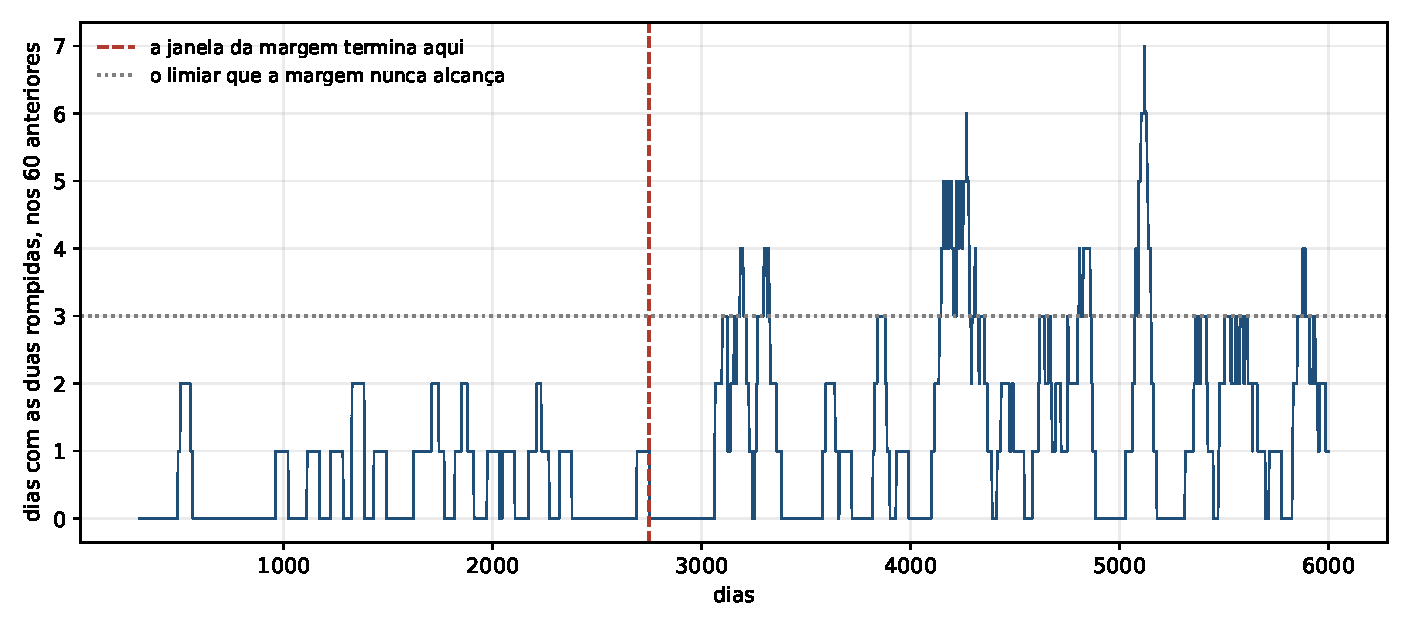
\includegraphics[width=\linewidth]{figuras/E09_dependencia_vigiada_1.pdf}
  \caption{A contagem conjunta, dia a dia, com o dia da mudança e o limiar do meio. Antes da
    linha, a série é quase colada no chão; depois, os picos ficam mais altos e mais próximos. A
    mudança não aparece como degrau: aparece como mais dentes na linha, e quem procura um salto na
    figura não o encontra.}
  \label{fig:vizinhanca}
\end{figure}

\section{O controle}

Falta o controle que separa o que é do dado do que é do instrumento. O orçamento da
\cref{tab:vizinhanca} não foi suposto: ele foi medido no mundo em que o par \textbf{não} muda. Com o
limiar três, esse mundo alarmou em \numVizinhancaControleAlarmouPct\% dos mundos sorteados, o que
é a taxa que o limiar de fato entrega --- e é contra ela que a latência se lê.

Sem essa medição, um limiar escolhido no olho pareceria silencioso e pareceria rápido, porque as
duas coisas seriam afirmações sobre nada.

\section{O que fica}

Fica a primeira resposta da travessia, e ela é limpa: \textbf{o vigia de margem não vê dependência} ---
não por defeito de calibração, mas porque a mudança não está em nenhuma das séries que ele lê. O
instrumento que vê existe, foi medido aqui, e cobra meses.

Fica também a forma que a travessia tem, e que as outras quatro perguntas dela vão repetir: pegar
o objeto de uma família e medi-lo com o instrumento de outra. É onde a lista do contrato cresce
sozinha, e é onde este livro deixa de ter uma gaveta por assunto.

E fica o fracasso seguinte, que é o que o capítulo anterior já havia encomendado e este não
resolve. Saber que a dependência é cara não diz o que fazer com ela. A pergunta que sobra é de
desenho: que intervenção distinguiria as explicações que sobreviveram, quanto custaria em dado que
não existe, e se ela é sequer possível. Um experimento que não se pode fazer é uma opinião com
instrumentos; um que se pode fazer é uma medida. A travessia ainda tem de enfrentar essa
diferença.
